% Created 2020-04-10 Fri 12:38
% Intended LaTeX compiler: pdflatex
\documentclass{article}
\usepackage[utf8]{inputenc}
\usepackage[T1]{fontenc}
\usepackage{graphicx}
\usepackage{grffile}
\usepackage{longtable}
\usepackage{wrapfig}
\usepackage{rotating}
\usepackage[normalem]{ulem}
\usepackage{amsmath}
\usepackage{textcomp}
\usepackage{amssymb}
\usepackage{capt-of}
\usepackage{hyperref}
\date{\today}
\title{}
\hypersetup{
 pdfauthor={},
 pdftitle={},
 pdfkeywords={},
 pdfsubject={},
 pdfcreator={Emacs 26.3 (Org mode 9.3.6)}, 
 pdflang={English}}
\begin{document}

\tableofcontents

\section{Totest list}
\label{sec:orgd5c2049}
\begin{enumerate}
\item Bitmaniplation\hfill{}\textsc{BIT}
\label{sec:org6adf0fe}
\begin{enumerate}
\item Bit maniplation of Inode\hfill{}\textsc{INODE}
\label{sec:orga93b7a7}
\begin{center}
\begin{tabular}{lllllll}
Test Stragity & Test Number & Descritpion & Input & Expected Output & Actual Output & Pass/Fail\\
\hline
 &  &  & Stream of 114 bits & Create an inode object, by the spefied 114 bits. &  & \\
 &  &  & Inode object & write as a stream of 114 bits &  & \\
\end{tabular}
\end{center}



\item Bit maniplation of Directory\hfill{}\textsc{DIR}
\label{sec:orgf4db9a5}
\begin{center}
\begin{tabular}{lllllll}
Test Stragity & Test Number & Descritpion & Input & Expected Output & Actual Output & Pass/Fail\\
\hline
 &  &  & Stream of 4096 bits & Create an directory object, by the spefied 4096 bits. &  & \\
 &  &  & directory object & write as a stream of 4096 bits &  & \\
\end{tabular}
\end{center}
\end{enumerate}


\item Setting up the drives
\label{sec:orgde2e093}
\begin{enumerate}
\item File system scope\hfill{}\textsc{FS}
\label{sec:orge66d38d}
Error MEssages are sent to osErrMsg
\begin{enumerate}
\item FS\textsubscript{Boot}
\label{sec:org405506d}
\begin{center}
\begin{tabular}{lllllll}
Test Stragity & Test Number & Descritpion & Input & Expected Output & Actual Output & Pass/Fail\\
\hline
 &  &  & Success NoDisk & The external disk does not exist, creates it &  & \\
 &  &  & Success Disk & The external disk does  exist, clone it to wroking test and verify &  & \\
 &  &  & Failure Disk & The external disk does  exist, clone it to wroking test and verify, but fails, restuling in E\textsubscript{FILE}\textsubscript{BOOT} &  & \\
\end{tabular}
\end{center}

\item FS\textsubscript{Sync}
\label{sec:org34eefaa}
\begin{center}
\begin{tabular}{lllllll}
Test Stragity & Test Number & Descritpion & Input & Expected Output & Actual Output & Pass/Fail\\
\hline
 &  & Saves the workign disk to external disk & Working disk and external disk & Copy working disk to external disk &  & \\
\end{tabular}
\end{center}
\item FS\textsubscript{Reset}
\label{sec:org670414f}
\begin{center}
\begin{tabular}{lllllll}
Test Stragity & Test Number & Descritpion & Input & Expected Output & Actual Output & Pass/Fail\\
\hline
 &  &  & File System is unavaible to write till fs\textsubscript{BOOT} & The file system is unable to be access til FS\textsubscript{Boot} is claled. Any attmpt to do so will result in E\textsubscript{INVALID}\textsubscript{ACCESS}\textsubscript{ATTEMPT} &  & \\
 &  &  & Attmpt to access filesystem before/after FS\textsubscript{Reset} & Access Stuff/E\textsubscript{INVALID}\textsubscript{ACCESS}\textsubscript{ATTEMPT} &  & \\
 &  &  & Attmpt to access filestyem before/after FS\textsubscript{Boot} & E\textsubscript{INVALID}\textsubscript{ACCESS}\textsubscript{ATTEMPT}/Access Stuff &  & \\
\end{tabular}
\end{center}
\end{enumerate}
\item Disk Scope\hfill{}\textsc{DS}
\label{sec:org65028ce}
Error MEssages are sent to diskErrMsg
\begin{enumerate}
\item DISK\textsubscript{SETUP} and Save
\label{sec:org806e3fd}
\begin{center}
\begin{tabular}{lllllll}
Test Stragity & Test Number & Descritpion & Input & Expected Output & Actual Output & Pass/Fail\\
\hline
 &  &  & int DISK\textsubscript{INIT}() & Run before disk ops take place. All sectors are all zeros, and you create he superblcok and the root direcotry. Called during FS\textsubscript{Boot} &  & \\
 &  &  & int Disk\textsubscript{Load} & When booting a Disk, you send External Disk -> working Disk. Called during FS\textsubscript{Boot} &  & \\
 &  &  & int Disk\textsubscript{Save} & Called by FS\textsubscript{Sync}, send Working Disk -> External Disk. &  & \\
\end{tabular}
\end{center}
\item DISK Write
\label{sec:org0accb53}
\begin{center}
\begin{tabular}{lllllll}
Test Stragity & Test Number & Descritpion & Input & Expected Output & Actual Output & Pass/Fail\\
\hline
 &  &  & Buffer is of SIZE\textsubscript{SEctor} & If not, than return E\textsubscript{WRITE}\textsubscript{INVALID}\textsubscript{PARAM} &  & \\
 &  &  & Buffer is nonNull & If not, than return E\textsubscript{WRITE}\textsubscript{INVALID}\textsubscript{PARAM} &  & \\
 &  &  & Sector paramter is out of boudns & retrun E\textsubscript{WRITE}\textsubscript{INVALID}\textsubscript{PARM} &  & \\
 &  &  & Sector has data being written to it & Write the Buffer to Sector. &  & \\
\end{tabular}
\end{center}
\item DISK Read
\label{sec:org45858cb}
\begin{center}
\begin{tabular}{lllllll}
Test Stragity & Test Number & Descritpion & Input & Expected Output & Actual Output & Pass/Fail\\
\hline
 &  &  & Buffer is of SIZE\textsubscript{SEctor} & If not, than return E\textsubscript{READ}\textsubscript{INVALID}\textsubscript{PARAM} &  & \\
 &  &  & Buffer is nonNull & If not, than return E\textsubscript{READ}\textsubscript{INVALID}\textsubscript{PARAM} &  & \\
 &  &  & Sector paramter is out of boudns & retrun E\textsubscript{READ}\textsubscript{INVALID}\textsubscript{PARM} &  & \\
 &  &  & Sector has data being read from to it & Write the Sector to Buffer. &  & \\
\end{tabular}
\end{center}
\end{enumerate}
\end{enumerate}
\item Setting up Directories and files
\label{sec:org3d724d0}
\begin{enumerate}
\item getFilePath(string path) and getDirPath(string path)
\label{sec:org9a2ce2d}
\begin{center}
\begin{tabular}{lllllll}
Test Stragity & Test Number & Descritpion & Input & Expected Output & Actual Output & Pass/Fail\\
\hline
 &  &  & String path & given path, get the inode assoicated with it & -1 if that path is not found with the correct type & \\
\end{tabular}
\end{center}

\item DIR\hfill{}\textsc{DIR}
\label{sec:orge408586}
\begin{enumerate}
\item Directory Create
\label{sec:org9375d1f}
\begin{center}
\begin{tabular}{llllllll}
Test Stragity & Test Number & Descritpion & Input & Expected Output & Actual Output & Pass/Fail & \\
\hline
 &  &  & Go to parent path File does not exist & Create directory at paretn directory &  &  & \\
 &  &  & Go to parent path Failure Exist & Get the file of the parent path, and once you do that, you see hte file \textbf{Path} already exist. Than, you return E\textsubscript{DIR}\textsubscript{CREATE} &  &  & \\
 &  &  & Go to parent path Failure Bad Path & Get the file of the parent path, but you the parent path doesn't exist. Than, you return E\textsubscript{DIR}\textsubscript{CREATE} &  &  & \\
 &  &  & Path exceeds 256 characters & If the supposed path is greater than 256 characters, or 2048 bits, return E\textsubscript{TOO}\textsubscript{LONG}\textsubscript{PATH} &  &  & \\
\end{tabular}
\end{center}
\item Directory Size/Read
\label{sec:org72e4d51}
\begin{center}
\begin{tabular}{llllllll}
Test Stragity & Test Number & Descritpion & Input & Expected Output & Actual Output & Pass/Fail & \\
\hline
 &  &  & Return the number of bytes in a path with Dir\textsubscript{Size}() & These two functions work in tandem, and as such, have to play nice. &  &  & \\
 &  &  & DIR\textsubscript{SIZE}() works & Gets a size of the direcotry, and sets hte buffer to appoperaite size. Note that each entry in a direcotry is 20 bytes &  &  & \\
 &  &  & DIR\textsubscript{READ} Success & The buffer is of appoperaite size, adn as such, you can write each inode to it. &  &  & \\
 &  &  & DIR\textsubscript{READ} Faiure Size too small & The buffer is of too small size, return E\textsubscript{BUFFER}\textsubscript{TOO}\textsubscript{SMALL} &  &  & \\
 &  &  & DIR\textsubscript{READ} Faiure Dir no eixst & directory does not exist, return E\textsubscript{DIR}\textsubscript{NO}\textsubscript{EXIST} &  &  & \\
\end{tabular}
\end{center}
\end{enumerate}
\item Files\hfill{}\textsc{FILE}
\label{sec:org2a9827b}
\begin{enumerate}
\item Create/Open and Close
\label{sec:org92d4b98}
\begin{center}
\begin{tabular}{llllllll}
Test Stragity & Test Number & Descritpion & Input & Expected Output & Actual Output & Pass/Fail & \\
\hline
 &  &  & File\textsubscript{Create}(string File) Success & Create a file at the path, with size 0. &  &  & \\
 &  &  & File\textsubscript{Create}(string File) Failure already exist & Failed at creating a file, due to there already being a file. Return E\textsubscript{FILE}\textsubscript{CREATE} &  &  & \\
 &  &  & File\textsubscript{Create}(string File) Failure max file size & The filessystem reaches max files. Return E\textsubscript{FILE}\textsubscript{CREATE} &  &  & \\
 &  &  & Path exceeds 256 characters & If the supposed path is greater than 256 characters, or 2048 bits, return E\textsubscript{TOO}\textsubscript{LONG}\textsubscript{PATH} &  &  & \\
 &  &  & File\textsubscript{Open} success & File doe exist and doesnt' exceed files open limit &  &  & \\
 &  &  & File\textsubscript{Open} Fialure noExist & File does not exist, return E\textsubscript{NO}\textsubscript{SUCH}\textsubscript{FILE} &  &  & \\
 &  &  & File\textsubscript{Open} Fialure alreadyOpen & File already is opened. return E\textsubscript{FILE}\textsubscript{ALREADY}\textsubscript{OPEN} &  &  & \\
 &  &  & File\textsubscript{Open} Fialure too many open files & File does  exist, but there's too many open files. return E\textsubscript{TOO}\textsubscript{MANY}\textsubscript{OPEN}\textsubscript{FILES} &  &  & \\
 &  &  & File\textsubscript{CLose}(int fd) Success & Close file in open file table, with fd. &  &  & \\
 &  &  & File\textsubscript{CLose}(int fd) Failure & File is not in open file table, return E\textsubscript{CLOSE}\textsubscript{BAD}\textsubscript{FD} &  &  & \\
\end{tabular}
\end{center}
\item File Read, write
\label{sec:orgfb79fa3}
\begin{center}
\begin{tabular}{llllllll}
Test Stragity & Test Number & Descritpion & Input & Expected Output & Actual Output & Pass/Fail & \\
\hline
 &  &  & File\textsubscript{Read}(int fd, string fuffer, int size) Success & check Open file, go to current posistion in file, than read from current possiton to size/end of file. Than have current file posistion &  &  & \\
 &  &  & File\textsubscript{Read}(int fd, string fuffer, int size) Failure not open & File is not in open file table, and thus, return E\textsubscript{READ}\textsubscript{BAD}\textsubscript{FD}. &  &  & \\
 &  &  & File\textsubscript{Write}(int fd, string fuffer, int size) Success & Write to a file from buffer, from teh buffer. Current file offset shold be by size. &  &  & \\
 &  &  & File\textsubscript{Write}(int fd, string fuffer, int size) Failure not open & Write to a file from buffer, from teh buffer. Current file offset shold be by size. Return E\textsubscript{WRITE}\textsubscript{BAD}\textsubscript{FD} &  &  & \\
 &  &  & File\textsubscript{Write}(int fd, string fuffer, int size) Failure no space left & While writing, if you find there's no more space in teh disk, return E\textsubscript{NO}\textsubscript{SPACE} &  &  & \\
 &  &  & File\textsubscript{Write}(int fd, string fuffer, int size) Failure maximum file size & While writing, if you find there's the file takes up more than 10 data blcoks, return E\textsubscript{FILE}\textsubscript{TOO}\textsubscript{BIG} &  &  & \\
\end{tabular}
\end{center}
\end{enumerate}
\end{enumerate}

\item Seek and unLink
\label{sec:org04671c6}
\begin{enumerate}
\item File\textsubscript{Seek} and Dir/File\textsubscript{UnLink}\hfill{}\textsc{FILE:DIR}
\label{sec:org0a08fd7}

\begin{center}
\begin{tabular}{llllllll}
Test Stragity & Test Number & Descritpion & Input & Expected Output & Actual Output & Pass/Fail & \\
\hline
 &  &  & File\textsubscript{Unlink}(String File) & Remove file in inode lbock, and freeing up any datablocks/indoes the file used. &  &  & \\
 &  &  & File\textsubscript{Unlink}(String File) but no such file & File does not exist. Return E\textsubscript{CLOSE}\textsubscript{BAD}\textsubscript{FD} &  &  & \\
 &  &  & File\textsubscript{Unlink}(String File) but file is already opened & File is currenlty opened. Return E\textsubscript{File}\textsubscript{IN}\textsubscript{Use} &  &  & \\
 &  &  & Dir\textsubscript{Unlink}(String File) Directory is  empty & Remove file from parent inode pointers, and htan free up the inode/data blocks. &  &  & \\
 &  &  & Dir\textsubscript{Unlink}(String File) Directory is not empty & Return E\textsubscript{DIR}\textsubscript{NOT}\textsubscript{EMPTY} &  &  & \\
 &  &  & Dir\textsubscript{Unlink}(String File) Direcotry is root & return E\textsubscript{DEL}\textsubscript{ROOT}\textsubscript{DIR} &  &  & \\
 &  &  & Dir\textsubscript{Unlink}(String File) Direcotry does not exist & retur E\textsubscript{DIR}\textsubscript{NON}\textsubscript{EXIST} &  &  & \\
 &  &  & File\textsubscript{Seek}(int fd, int offset) & File's posstiion is chnaged by the offset &  &  & \\
 &  &  & File\textsubscript{Seek}(int fd, int offset) Out of bounds & Offset is negative/exceeds file size. Return E\textsubscript{SEEK}\textsubscript{OUT}\textsubscript{OF}\textsubscript{BOUNDS} &  &  & \\
 &  &  & File\textsubscript{Seek}(int fd, int offset) bad fd & File isn't open. Return out of bounds &  &  & \\
\end{tabular}
\end{center}
\end{enumerate}
\end{enumerate}

\section{Algorithm/Code}
\label{sec:orgdb66fee}
\begin{enumerate}
\item Whoel Porgram decompsiostion
\label{sec:org8545936}
This is an outline/code of how the whole program will be. 
\item Bit Parsing/Data Strucutre\hfill{}\textsc{BIT}
\label{sec:orgfc7f182}
\begin{itemize}
\item As we are writing bits, we have to format the disk to be able to read and write bits.
\item SUPERBLOCK | indoebitmap | datablock bitmap | sequence of indoes | sequence of datablcoks = 1000
\item the sequence of indoes will ahve 3 sectors, due to each indoe being able to represtn 35 inodes.
\item The rest of the space, 994 sectors, are for teh databock block.
\end{itemize}

\begin{enumerate}
\item inode
\label{sec:org923345f}
\begin{description}
\item{writeBitStream()} Write teh type, size and allociation, by reversing the blwo opeariton

\item{readBitStream()} read the type, size and allcioation by folowing the following processess

\item There are 4 indoes within a inode sector. The makeup totals to 114 bits.
\begin{description}
\item{1 bit } for which type of inode this is.
\item{13 bits} (or 1.625 bytes) for representing the size of datablocks
\item{100 bits} 10 seqeunces of 10 bits for reprsenting the location. note that all 1s mean that this is not allociated
\end{description}

\item This results of 106 of useless data, and 3990 of useful data. Since there are 35 inodes in a sector, we split it up into an array, with each piece being a substr of 114 bits.

\item The function below is a method ofreading it. Note it doesn't return anything. Maybe i'll try to do that thing where i have an inlnie function and do it there.

\item Anotehr note: there'll be 35 inodes withn a sector, so the spliting of that by 114 is left to futrue zak.

\item Writing it to bitstream is simple. if need be write a funciton for it.

\begin{verbatim}
#include<iostream>
#include<bitset>
using namespace std;
// Note in babel mode this will be incorrect

void readBitDataInode(string Inode){
// Type // Size // 10*10 of which bits are allociated to it.

    // This little test is used to demonstrate values used to finding where to substring
    /*
    string test= "11111NNNNN22222NNNNN33333NNNNN44444NNNNN55555NNNNN66666NNNNN77777NNNNN88888NNNNN99999NNNNN00000NNNNNSSSSSSSSSSSSST";
    cout << test.substr(0,100) << endl; //Which are allcoiated
    cout << test.substr(100,13) << endl; //Size
    cout << test.substr(113,1) << endl; //Type
    for(int i=0; i<10; i++){ 
	cout << test.substr(i*10,10) << endl;  // used to show how to splti the function
    }
    */


	uint alloc[10];
	for(int i=0; i<10; i++){
		bitset<10> temp(Inode.substr(i*10, 10));
		cout << temp << '\t' << temp.to_ulong() << endl;
		alloc[i]=temp.to_ulong();
	}
	uint size;
	bitset<13> temp2(Inode.substr(100,13));
	size=temp2.to_ulong();

	bool type;
	bitset<1> temp3(Inode.substr(113,1));
	cout << temp3 << endl;
	type=temp3.to_ulong();

	cout << size << '\t' << type << endl;
}

int main(){
	string test= "000000000011111111110000000000111110000000000111111010101001000000000110000000000000100000001000010011111111111110";
	readBitDataInode(test);
	cout << "WOW";
}
\end{verbatim}
\end{description}


\item datablock
\label{sec:org5c5a109}
\begin{itemize}
\item Datablocks are disgshiustehd by two types: file and directory
\item the type of the datablock is denoted by teh inode, not the directory.
\item For directory, tehre is a 20 bytes/160 bits, which are
\begin{description}
\item{16 bytes/128 bits} file name. 15 characters PLUS 1 for end of string, so it's mroe of 15 characters
\item{4 byte/32 bits} inode that shows which file/driectory this is.
\end{description}
\item This means that dictionaries cna have 25 files in a a sector, but 250 files/directories overall.
\item This doesn't have the case, of half a directoriy's infroamtion being in one datablcok, and the other half being in another datablock. THat isn't consdiered.
\begin{verbatim}
using namespace std;
void readDir(string TestString){
    bitset<64> inode(TestString.substr(0,4));
    cout << inode.to_ulong() << endl;
    char temp[10];
    for(int i=0; i<8; i++){
	    bitset<16> temp(TestString.substr(4+i*16,16));
	    cout << (char)temp.to_ulong() << endl;

    }

}

int main(){
/*
	string temp1="iiii11111111111111112222222222222222333333333333333344444444444444445555555555555555666666666666666677777777777777778888888888888888";
	for(int i=0; i<8; i++){
	    cout << temp1.substr(4+i*16,16) << endl;
	}
*/
	/*readDir("111110000000000000001000000000000000100000000000000010000000000000001000000000000000100000000000000010000000000000001000000000000000");*/
	readDir("111100000000010000010000000001000010000000000100001100000000010001000000000001000101000000000100011000000000010001110000000001001000");
}

\end{verbatim}
\end{itemize}


\item bitmap of indoe/datablock
\label{sec:org1c09642}
\begin{itemize}
\item this is just a bitmap, used to keep trakc of which indoes are allociated and which datablocks are allociated.
\end{itemize}
\item Sector/Root Inode
\label{sec:orgbd79749}
\begin{itemize}
\item A sector is a collection of a superblock, bitmaps for in use indoes and datablocks, a sqeunce of indoes, and a sequence of datablocks.  However, this information HAS TO BE CONVERETD to that. Otehrwise, a sector is just an array of bitsets of 4096 bits.
\item However, the sector converts it's concats to usuable datasturcutres. After each file/directory operation, it saves the stuff to workign directory. Than, working directory saves it stuff to external disk when FS\textsubscript{SYNC}() is made.
\item The disks are just a bitset array of 4096 bits, with 1000 elements in each.
\item The root inode is the indoe that represtns nothing. This is a special variable, as to not have to find out what it is on disk tediously.
\end{itemize}

\begin{verbatim}
std::bitset<4096> ExtDisk[1000];
std::bitset<4096> WorkDisk[1000];
\end{verbatim}
\end{enumerate}

\item File System\hfill{}\textsc{FS}
\label{sec:org42e4b43}
\begin{description}
\item{FS\textsubscript{BOOT}()} Called when booting filesystem/after a FS\textsubscript{RESET}()
\begin{center}
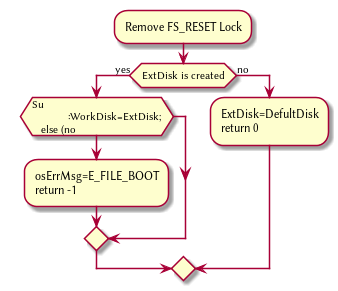
\includegraphics[width=.9\linewidth]{Plant/FS_BOOT.png}
\end{center}

\item{FS\textsubscript{Sync}} Copys the working disk to external disk
\begin{center}
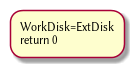
\includegraphics[width=.9\linewidth]{Plant/FS_SYNC.png}
\end{center}

\item{FS\textsubscript{RESET}()} Stops the filesystem from ebing access, by placing a lock on it. 
\begin{center}
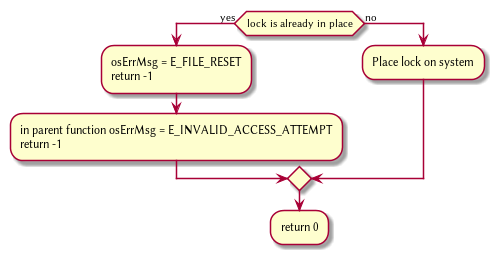
\includegraphics[width=.9\linewidth]{Plant/FS_RESET.png}
\end{center}
\end{description}


\item File Access\hfill{}\textsc{FILE}
\label{sec:org6d0d50a}
\begin{description}
\item{int getDirPath(string path)} Helper function, used to get the directory given a path.
\begin{description}
\item{Ouptut} inode number of where it is, or -1 if it's not found.
\begin{center}
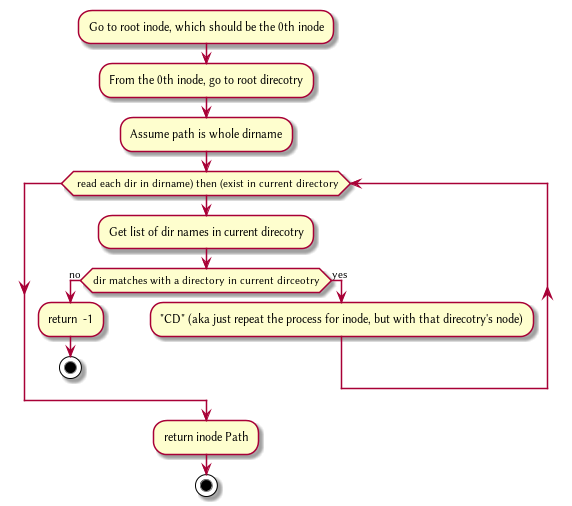
\includegraphics[width=.9\linewidth]{Plant/getDirPath.png}
\end{center}
\end{description}

\item{int getFilePath(string path)} Helper function, used to get the file given a path.
\begin{description}
\item{Ouptut} inode number of where it is, or -1 if it's not found.
\begin{center}
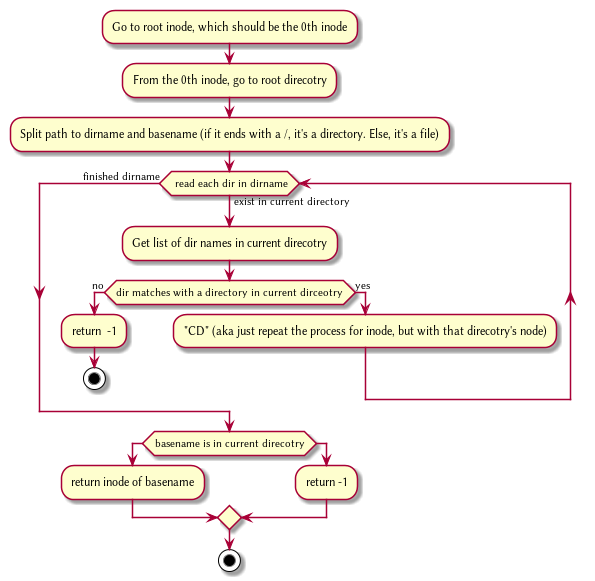
\includegraphics[width=.9\linewidth]{Plant/getFilePath.png}
\end{center}
\end{description}

\item{File\textsubscript{Create}(string path)} Create a new file at path. There is a check to see if that file already exist, and if there's a free datablock for it.
\begin{center}
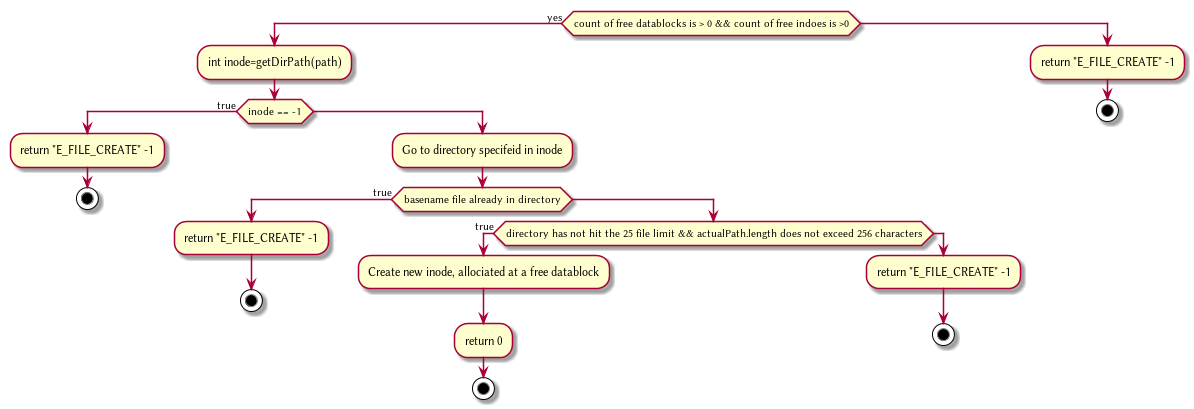
\includegraphics[width=.9\linewidth]{Plant/FileCreate.png}
\end{center}
\end{description}


\begin{description}
\item{File\textsubscript{Open}(string path)} returns the file descriptor of the file, which can be used to read and write to it.
\begin{center}
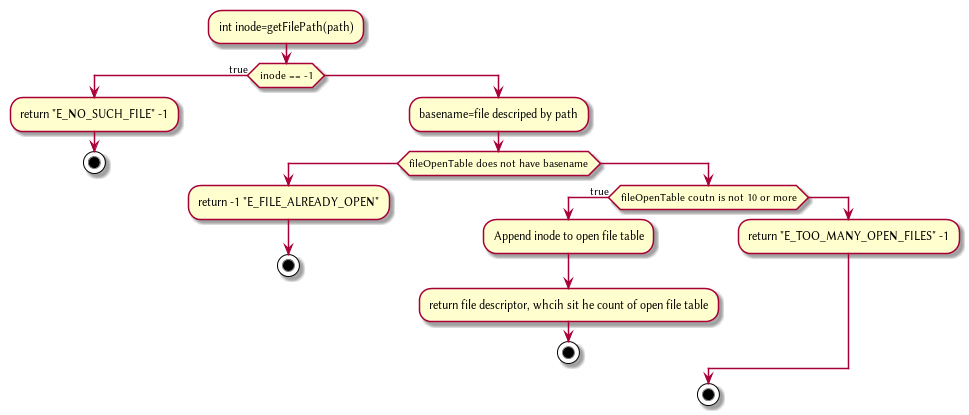
\includegraphics[width=.9\linewidth]{Plant/FileOpen.png}
\end{center}
\item{File\textsubscript{Read}(int fd, string buffer, int size IN BYTES)} Buffer reads size from the file in fd. Note the file in open file table shuold move by size
\begin{center}
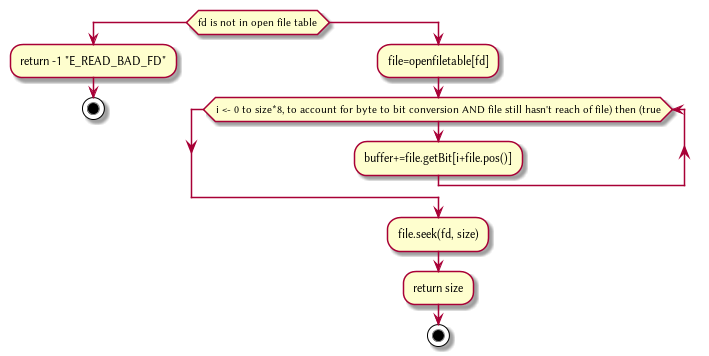
\includegraphics[width=.9\linewidth]{Plant/FileREAD.png}
\end{center}
\item{File\textsubscript{Write}(int fd, string buffer, int size IN BYTES)} Write from buffer to the file. NOTE SIZE HAS TO BE CONSISNET. If it's not, stop the program
\begin{center}
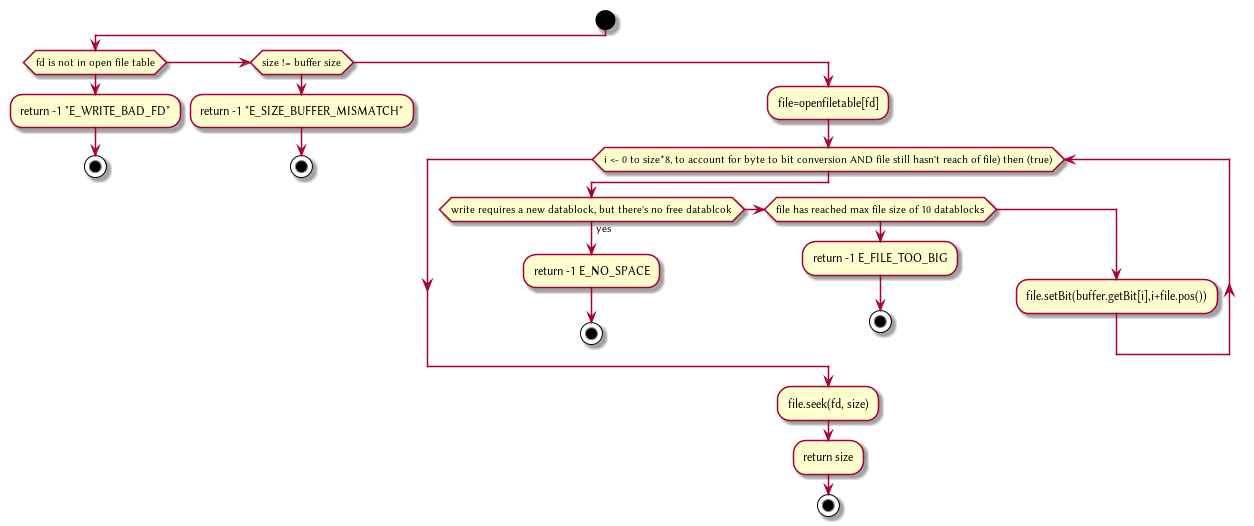
\includegraphics[width=.9\linewidth]{Plant/FileWrite.png}
\end{center}

\item{File\textsubscript{Seek}(int fd, int offset)} move the file forward  by offset.
\begin{center}
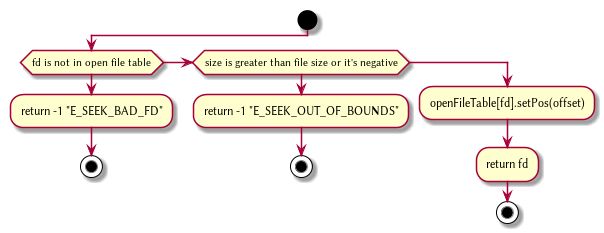
\includegraphics[width=.9\linewidth]{Plant/FileSeek.png}
\end{center}

\item{File\textsubscript{Close}(int fd)} Remove file from table
\begin{center}
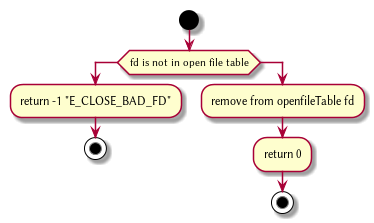
\includegraphics[width=.9\linewidth]{Plant/FileClose.png}
\end{center}

\item{File\textsubscript{UnLink}(string path)} Delete file from the filesystem.
\begin{center}
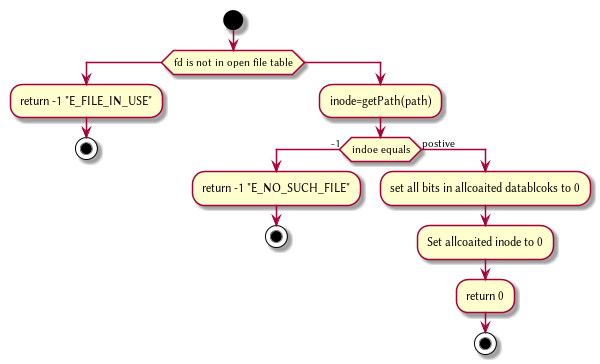
\includegraphics[width=.9\linewidth]{Plant/FileDelete.png}
\end{center}
\end{description}

\item Directory\hfill{}\textsc{DIR}
\label{sec:orgf3a7d33}
\begin{description}
\item{Dir\textsubscript{Create}(string path)} Create directory at path
\begin{center}
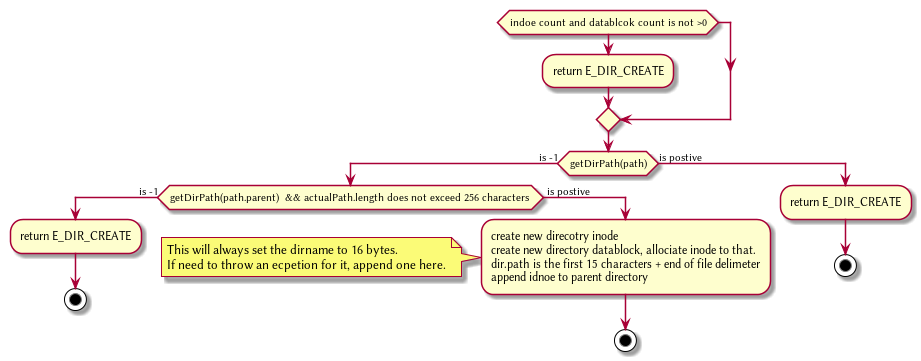
\includegraphics[width=.9\linewidth]{Plant/DirCreate.png}
\end{center}

@startuml

\item{Dir\textsubscript{Read}(string path, string buffer, itn size)} Read the contents of a directory.
\begin{center}
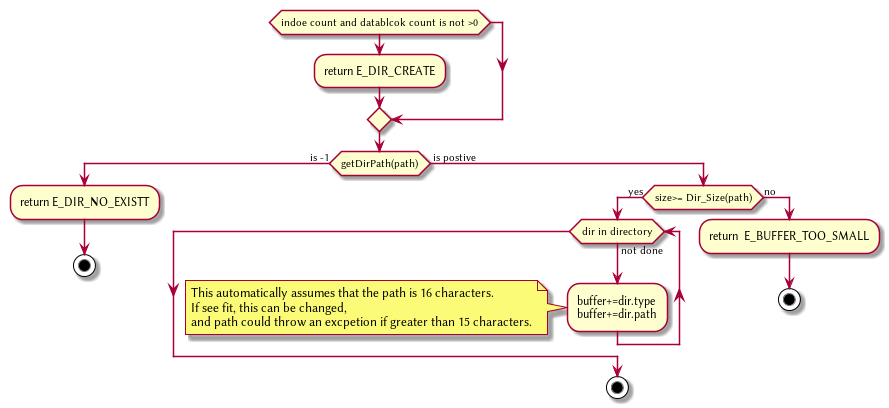
\includegraphics[width=.9\linewidth]{Plant/DirRead.png}
\end{center}
\item{Dir\textsubscript{Unlink}(string path)} Remove file from drive
\begin{center}
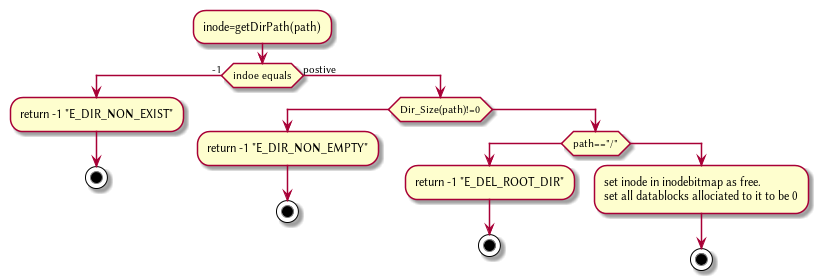
\includegraphics[width=.9\linewidth]{Plant/DirUnlink.png}
\end{center}
\end{description}

\item Disk\hfill{}\textsc{DISK}
\label{sec:org8661781}

\begin{description}
\item{DISK\textsubscript{INIT}()} Set all the data in the disk to be 0
\begin{center}
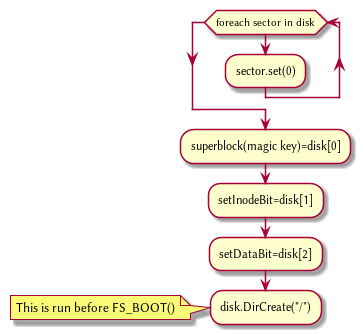
\includegraphics[width=.9\linewidth]{Plant/DIskInit.png}
\end{center}

\item{DISK\textsubscript{LOAD}()} Save external disk to workign disk. Done when booting. 

\begin{center}
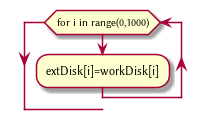
\includegraphics[width=.9\linewidth]{Plant/DIskLoad.png}
\end{center}

\item{DISK\textsubscript{SAVE}()} Save working disk to loading. Called by FS\textsubscript{SYNC}()
\end{description}
\begin{center}
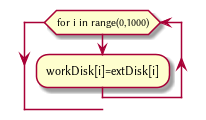
\includegraphics[width=.9\linewidth]{Plant/DIskSave.png}
\end{center}

\begin{description}
\item{DISK\textsubscript{WRITE}(int sector, string buffer)} Write from buffer to disk.

\begin{center}
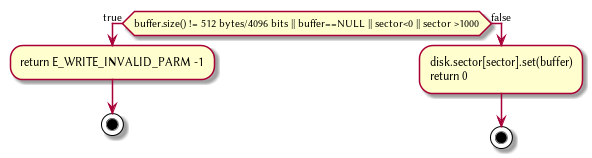
\includegraphics[width=.9\linewidth]{Plant/DiskWrite.png}
\end{center}
\end{description}



\begin{description}
\item{DISK\textsubscript{Read}(int sector, string buffer)} read from sector to buffer

\begin{center}
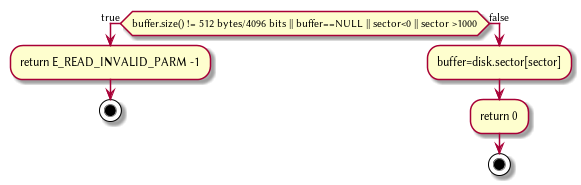
\includegraphics[width=.9\linewidth]{Plant/DiskREAD.png}
\end{center}
\end{description}
\end{enumerate}
\end{document}